%------------------------------------------------------------------------------
% Beginning of journal.tex
%------------------------------------------------------------------------------
%
% AMS-LaTeX version 2 sample file for journals, based on amsart.cls.
%
%        ***     DO NOT USE THIS FILE AS A STARTER.      ***
%        ***  USE THE JOURNAL-SPECIFIC *.TEMPLATE FILE.  ***
%
% Replace amsart by the documentclass for the target journal, e.g., tran-l.
%
\documentclass{amsart}

%     If your article includes graphics, uncomment this command.
\usepackage{graphicx}
\usepackage[latin1]{inputenc}
\usepackage[brazil]{babel}
\usepackage{marginnote}
\usepackage[pdftex,bookmarks,colorlinks]{hyperref}
\usepackage{bm}

\theoremstyle{theorem}
\newtheorem{teorema}{Teorema}[section]
\newtheorem{proposicao}{Proposi\c{c}\~{a}o}[section]
\newtheorem{corolario}{Corol\'{a}rio}[section]
\newtheorem{lema}{Lema}[section]

\theoremstyle{definition}
\newtheorem{definicao}{Defini\c{c}\~{a}o}[section]
\newtheorem{notacao}{Nota\c{c}\~{a}o}[section]

\theoremstyle{remark}
\newtheorem{remark}{Remark}[section]
\newtheorem{conjectura}{Conjectura}[section]

\numberwithin{equation}{section}

%\newcommand{\mn}[1]{#1 \marginnote{\footnotesize{#1}}}
%\newcommand{\mnn}[1]{\marginnote{\footnotesize{#1}}}


\newcommand{\mn}[1]{#1 \marginpar[\begin{flushright} \footnotesize{#1}\end{flushright}]{\begin{flushleft}\footnotesize{#1}\end{flushleft}}}
\newcommand{\mnn}[1]{\marginpar[\begin{flushright} \footnotesize{#1}\end{flushright}]{\begin{flushleft}\footnotesize{#1}\end{flushleft}}}

\newcommand{\im}[1]{\mathrm{Im}(#1)}
\newcommand{\ex}[1]{\mathrm{ex}(#1)}
\renewcommand{\mod}[1]{\quad(\mathrm{mod}\;#1)}
\newcommand{\prob}[1]{\mathbb{P}[#1]}
\newcommand{\E}[1]{\mathbb{E}[#1]}
\newcommand{\N}{\mathbb{N}}
\newcommand{\Q}{\mathbb{Q}}
\newcommand{\R}{\mathbb{R}}
\newcommand{\bt}{\mbox{\boldmath{$\theta$}}}
\newcommand{\tr}[1]{\mathrm{tr}(#1)}

\newcommand{\dubb}[1]{[\![#1]\!]}

%    Absolute value notation
\newcommand{\abs}[1]{\lvert#1\rvert}

%    Blank box placeholder for figures (to avoid requiring any
%    particular graphics capabilities for printing this document).
\newcommand{\blankbox}[2]{%
  \parbox{\columnwidth}{\centering
%    Set fboxsep to 0 so that the actual size of the box will match the
%    given measurements more closely.
    \setlength{\fboxsep}{0pt}%
    \fbox{\raisebox{0pt}[#2]{\hspace{#1}}}%
  }%
}

\begin{document}

\title{Flag-\'{A}lgebras}

%    Information for first author
\author{Walner Mendon\c{c}a dos Santos\\}
%    Address of record for the research reported here
\address{Universidade Federal do Cear\'{a}}
%    Current address
%\curraddr{Department of Mathematics and Statistics, Case Western Reserve University, Cleveland, Ohio 43403}
\email{walner@alu.ufc.br}
%    \thanks will become a 1st page footnote.
%\thanks{The first author was supported in part by NSF Grant \#000000.}

%    Information for second author
\author{Fabricio Siqueira Benevides}
%\address{Universidade Federal do Cear\'{a}}
%\email{fabricio@mat.ufc.br}
%\thanks{Support information for the second author.}

%    General info
%\subjclass[2000]{Primary 54C40, 14E20; Secondary 46E25, 20C20}

\date{Outubro de 2013.}

%\dedicatory{This paper is dedicated to our advisors.}

\keywords{Combinat\'{o}ria, Flag-\'{a}lgebras}

\begin{abstract}
Notas de estudo.
\end{abstract}

\maketitle

\tableofcontents

\section{Introdu\c{c}\~{a}o}
Minhas principais refer\^{e}ncias s\~{a}o \cite{razborov,sudakov}.

\subsection{Nota\c{c}\~{a}o}
Introduziremos algumas nota\c{c}\~{o}es \emph{non-standard}. Assumiremos que as nota\c{c}\~{o}es can\^{o}nicas da teoria dos grafos s\~{a}o bem conhecidas. As principais nota\c{c}\~{o}es s\~{a}o oriundas da refer\^{e}ncia \cite{razborov}. Algumas poucas coisas foram acrescentadas para facilitar a compreens\~{a}o.

O conjunto de n\'{u}meros naturais $\{1,2,\ldots,n\}$ ser\'{a} denotado por $[n]$. Uma \mn{\emph{sunflower}} \index{sunflower} $(V_1,\ldots,V_k)$ com \emph{centro} $C$ \'{e} uma cole\c{c}\~{a}o finita de conjuntos $V_1,\ldots,V_k$ tais que $V_i\cap V_j = C$, para todo $i,j$ elementos distintos de $[k]$. Quando for conveniente explicitar o centro da sunflower, escreveremos $(V_1,\ldots,V_k;C)$. Os conjuntos $V_1,\ldots,V_k$ s\~{a}o as \mn{\emph{p\'{e}talas}} da sunflower.

Dado um grafo $G = (V,E)$, um subconjunto $V'\subseteq V$ induz um subgrafo em $G$ o qual denotamos por \mn{$G|_{V'}$}. Uma \mn{\emph{$r$-rotula\c{c}\~{a}o}} $\theta$ de um grafo $G$ \'{e} uma fun\c{c}\~{a}o injetiva $\theta: [r]\rightarrow V(G)$ (observe que para que $\theta$ seja injetiva, \'{e} necess\'{a}rio que $|G| \geq r$). O par $(G,\theta)=:R$ \'{e} dito ser um \mn{\emph{grafo rotulado}}. Quando $\theta$ \'{e} bije\c{c}\~{a}o, dizemos que $(G,\theta)$ \'{e} um \emph{grafo inteiramente rotulado}. Nota\c{c}\~{o}es \emph{standards} para grafos se mant\^{e}m para grafos rotulados. Por exemplo, $V(R) := V(G)$ e $|R| := |G|$. Denotamos por \mn{$G |_{\theta}$} o subgrafo induzido por $\theta([r])$, i.e., $G|_{\theta([r])}$. Quando dois grafos $G_1$ e $G_2$ forem isomorfos, denotaremos \mn{$G_1 \approx G_2$}. Dois grafos rotulados $R_1:= (G_1,\theta_1)$ e $R_2:=(G_2,\theta_2)$ s\~{a}o isomorfos quando $G_1\approx G_2$, $G_1|_{\theta_1} \approx G_2|_{\theta_2}$ e $\theta_1 \approx \theta_2$ (i.e., a rela\c{c}\~{a}o de adjac\^{e}ncia \'{e} preservada por r\'{o}tulos). E neste caso, escrevemos \mn{$R_1\approx R_2$}.

Iremos utilizar a tipografia $\mathbf{math\; bold\; face}$ para denotar objetos aleat\'{o}rios. E sempre, a menos de men\c{c}\~{a}o contr\'{a}ria, o espa\c{c}o de probabilidade envolvido ser\'{a} o espa\c{c}o de probabilidade discreto.

\subsection{Defini\c{c}\~{o}es}
No que segue, introduziremos as principais defini\c{c}\~{o}es de flag-\'{a}lgebras. Na refer\^{e}ncia \cite{razborov}, pode-se encontrar tais defini\c{c}\~{o}es em contextos mais gerais, onde s\~{a}o tratadas sob a perspectiva da teoria dos modelos. Contudo, a teoria dos grafos e hipergrafos \'{e} suficiente para uma boa introdu\c{c}\~{a}o e intui\c{c}\~{a}o dos conceitos envolvidos. Portanto, fazemos como \cite{sudakov}, apresentamos a teoria sob o contexto de grafos. Para o contexto de hipergrafos, os conceitos s\~{a}o semelhantes e iremos admitir que isto \'{e} claro.

\subsubsection{Tipo $\sigma$ e $\sigma$-flag}
Agora vamos a defini\c{c}\~{a}o do primeiro objeto da teoria de flag-\'{a}lgebras: o tipo. Neste ponto, chegamos num pequeno empasse, pois as nossas duas principais refer\^{e}ncias definem o tipo de maneira distintas, mas ainda assim, equivalentes. Seguiremos a defini\c{c}\~{a}o de \cite{sudakov}: um \mn{\emph{tipo}} $\sigma$ \'{e} um grafo inteiramente rotulado. Dizemos que $|\sigma|$ \'{e} o tamanho de $\sigma$.

Uma \mn{$\sigma$-\emph{flag}} \'{e} um grafo rotulado $F=(G,\theta)$ com $G|_\theta \approx \sigma$ (em particular, $\theta$ \'{e} uma $|\sigma|$-rotula\c{c}\~{a}o). Observe que para a boa defini\c{c}\~{a}o, devemos ter $|F|\geq |\sigma|$. Escreveremos \mn{$F|_V$} para denotar a flag induzida por $V\subseteq V(G)$, i.e., $(G|_V,\theta)$, desde que $\mathrm{Im}(\theta) \subseteq V$. Denotamos por \mn{$\mathcal{F}^{\sigma}$} a cole\c{c}\~{a}o de todas as $\sigma$-flag e definimos $\mathcal{F}^{\sigma}_{\ell} := \{F\in \mathcal{F}^{\sigma}; |F| = \ell \}$ \mnn{$\mathcal{F}^{\sigma}_{\ell}$}.

O tipo $(\emptyset,\mathrm{Id})$ sera denotado por $0$. Assim, \mn{$\mathcal{F}^{0}$} nada mais \'{e} do que o conjunto de todos os grafos n\~{a}o rotulados e, em particular, $\mathcal{F}^{0}_{\ell}$ \'{e} o conjunto dos grafos n\~{a}o rotulados com $\ell$ v\'{e}rtices. A $\sigma$-flag $(V(\sigma),\mathrm{Id})$, onde $\mathrm{Id}$ \'{e} a fun\c{c}\~{a}o identidade em $V(\sigma)$, ser\'{a} denotada por \mn{$1_\sigma$}, ou  por simplesmente $1$, quando $\sigma$ estiver claro a partir do contexto.

Dado $\tilde{F} \in \mathcal{F}^{\sigma}_{\tilde{\ell}}$ e $F \in\mathcal{F}^{\sigma}_{\ell}$, com $\tilde{\ell} \leq \ell$, escreveremos \mn{$\tilde{F} \preceq F$} para indicar que $\tilde{F}$ \'{e} uma \emph{subflag} de $F$, i.e., isomorfo a alguma flag do tipo $F|_{V}$, onde $V\subseteq{V(F)}$.

\subsubsection{Flag-densidades}
Seja $G$ e $H$ grafos com $|G| \leq |H|$. Seja \mn{$p(H;G)$} a probabilidade do evento $G|_\mathbf{V} \approx H$, onde $\mathbf{V}$ \'{e} um subconjunto de $V(G)$ com $|H|$ v\'{e}rtices escolhido de maneira aleat\'{o}ria e uniforme.

Fixe um tipo $\sigma$ com $k = |\sigma|$ e assuma que $\ell,\ell_1,\ldots,\ell_t \geq k$ s\~{a}o tais que
\begin{equation}\label{in1}
  \ell_1 + \cdots + \ell_t - k(t-1) \leq \ell,
\end{equation}
e que $F = (G,\theta) \in \mathcal{F}^{\sigma}$, $F_i \in \mathcal{F}^{\sigma}_{\ell} (1\leq i \leq t)$ s\~{a}o $\sigma$-flags. Escolha aleatoriamente e de maneira uniforme em $V(F)$ uma sunflower $(\mathbf{V}_1,\ldots,\mathbf{V}_t;C)$, sendo $C = \mathrm{Im} (\theta)$ e $|V_i| = \ell_i (1 \leq i \leq t)$. Gra\c{c}as a desigualdade~\ref{in1}, existe pelo menos uma sunflower, j\'{a} que
$$\left| \bigcup_{i=1}^{t} \bf{V}_i \right| = \ell_1 + \cdots + \ell_t - k(t-1) \leq \ell.$$
Denotamos por \mn{$p_\sigma(F_1,\ldots,F_t;F)$} a probabilidade de que $F|_{\bf{V_i}} \approx F_i$, para todo $i \in [t]$, i.e.,
\begin{equation}
  p_{\sigma}(F_1,\ldots,F_t;F) :=
   \mathbb{P} \left[\forall i \in [r],\; F|_{\bf{V_i}} \approx F_i\right].
\end{equation}
Algumas vezes ser\'{a} conveniente escrever \mn{$p(F_1,\ldots,F_t;F)$} ao inv\'{e}s de $p_{\sigma}(F_1,\ldots,F_t;F)$, desde que $\sigma$ esteja bem determinado pelo contexto.

%Observe que, para qualquer $\tilde{F}\in\mathcal{F}^{\sigma}_{\tilde{\ell}}$ e $F \in \mathcal{F}^{\sigma}_{\tilde{\ell}}$, com $\tilde{\ell} \leq \ell$, vale a identidade
%\begin{equation}
%  p_{\sigma}(\tilde{F};F) :=
%   \mathbb{P} \left[ \tilde{F}\preceq F \right].
%\end{equation}

\subsection{Propriedades}
Nesta se\c{c}\~{a}o, objetivamos apresentar as principais propriedades das flag-densidades.

\begin{proposicao}\label{prop1}
  \begin{itemize}
    \item[(a)] $p(1_{\sigma},F_1,\ldots,F_t;F) = p(F_1,\ldots,F_t;F)$ e $p(1_{\sigma};F) = 1$.
    \item[(b)] Se $F,F_1 \in \mathcal{F}^{\sigma}_{\ell}$, ent\~{a}o $p(F_1;F) = 1$, se $F = F_1$, e $p(F_1;F) = 0$, se $F \neq F_1$.
    \item[(c)] Seja $\pi$ uma $t$-permuta\c{c}\~{a}o. Ent\~{a}o $p(F_1,\ldots,F_t;F) = p(F_{\pi(1)},\ldots,F_{\pi(t)};F)$.
  \end{itemize}
  \begin{proof} Como todas s\~{a}o de f\'{a}cil verifica\c{c}\~{a}o, deixamos a cargo do leitor.\end{proof}
\end{proposicao}


\begin{remark}[Teorema da Probabilidade Total]\label{remark1}
  Seja $(\Omega,\Sigma,\mathbb{P})$ um espa\c{c}o de probabilidade. Se a sequ\^{e}ncia (finita ou enumer\'{a}vel) de eventos $\mathbf{B}_1,\mathbf{B}_2,\ldots \in \Sigma$ determinam uma parti\c{c}\~{a}o de $\Omega$, ent\~{a}o
  \begin{equation}
    \mathbb{P}[\mathbf{A}] = \sum_{i=1}^{\infty} \mathbb{P}[\mathbf{B}_i] \mathbb{P}[\mathbf{A}|\mathbf{B}_i] , \quad \forall \mathbf{A}\in \Sigma.
  \end{equation}
\end{remark}

At\'{e} agora, o que temos visto s\~{a}o defini\c{c}\~{o}es. E neste ponto, flag-\'{a}lgebras n\~{a}o parecem t\~{a}o interessante. De fato, a real aplicabilidade das flag-\'{a}lgebras reside em dois resultados fundamentais. Um deles fala sobre o comportamento assint\'{o}tico das flag-densidades em grafos suficientemente grandes, como veremos mais adiante. Outro \'{e} o seguinte resultado conhecido como \mn{\emph{regra da cadeia}}:

\begin{teorema}[Regra da Cadeia]
  Sejam $|\sigma| = k$, $F_i\in\mathcal{F}^{\sigma}_{\ell_i}\; (1\leq i \leq t)$, $1\leq s \leq t$, $F \in \mathcal{F}^{\sigma}_{\ell}$ e $\tilde{\ell} \leq \ell$ tais que
  \begin{equation}\label{RCin}
    \left\{
       \begin{array}{l}
         \ell_1 + \cdots + \ell_s - k(s-1) \leq \tilde{\ell}, \\
         \tilde{\ell} + \ell_{s+1} + \cdots + \ell_t - k(t-s) \leq \ell.
       \end{array}
     \right.
  \end{equation}
Ent\~{a}o
\begin{equation}\label{RC}
  p(F_1,\ldots,F_t;F) = \sum_{\tilde{F}\in\mathcal{F}^{\sigma}_{\tilde{\ell}}} p(F_1,\ldots,F_s;\tilde{F})\;p(\tilde{F},F_{s+1},\ldots,F_t;F).
\end{equation}
\end{teorema}

A ideia principal da prova deste teorema \'{e} usar o Remark~\ref{remark1}.

\begin{proof}  A fim de usarmos o Remark~\ref{remark1}, vamos determinar $\Omega$, $\bf{A}$, e os $\mathbf{B}_i$. Como para determinar o lado esquerdo da equa\c{c}\~{a}o~\ref{RC} precisamos sortear, em $F$, sunflowers $(\mathbf{V}_{1},\ldots,\mathbf{V}_{t})$ centradas em $C = \mathrm{Im}(\theta)$, temos que $\Omega$ \'{e} o conjunto de todas tais sunflowers.

A ideia \'{e}: ao inv\'{e}s de sortearmos uma sunflower do tipo $(\mathbf{V}_{1},\ldots,\mathbf{V}_{t}; C)$ em $F$, iremos primeiro sortear as $s$ primeiras p\'{e}talas em $\tilde{F}$, e ent\~{a}o iremos sortear as $t-s$ p\'{e}talas restantes em $F$ junto de uma p\'{e}tala $\mathbf{\tilde{V}}$ que eventualmente ir\'{a} induzir as $s$ primeiras p\'{e}talas em $F$, desde que $F|_{\tilde{V}} \approx \tilde{F}$.

Seja $\mathbf{A}$ o evento ``$\forall i\in[t], F|_{\mathbf{V}_i} \approx F_i$''. Para cada $\tilde{F}\in\mathcal{F}^{\sigma}_{\tilde{\ell}}$ (que, a priori, n\~{a}o sabemos se $\tilde{F} \preceq F$), considere $\mathbf{B}_{\tilde{F}}$ como o evento ``$\forall j\in[s], \tilde{F}|_{\mathbf{V}_j} \approx F_j$''. Observe que a primeira desigualdade em~\ref{RCin} nos permite determinar tal evento. Assim, temos que
\begin{eqnarray}
  p(F_1,\ldots,F_t;F) =  \mathbb{P}[\bf{A}], \label{pfRC1}\\
  p(F_1,\ldots,F_s;\tilde{F}) = \mathbb{P}[\mathbf{B}_{\tilde{F}}]\label{pfRC2}.
\end{eqnarray}
A primeira dessas equa\c{c}\~{o}es segue por defini\c{c}\~{a}o. J\'{a} a segunda segue observando que n\~{a}o interessa como s\~{a}o as p\'{e}talas $V_j$, para $j>s$, de modo que a probabilidade do evento ``$\forall j\in[s], \tilde{F}|_{\mathbf{V}_j} \approx F_j$'' diante de uma sunflower aleat\'{o}ria com $s$ p\'{e}talas $(\mathbf{V}_{1},\ldots,\mathbf{V}_{s}; C)$ \'{e} igual a probabilidade do evento ``$\forall j\in[s], \tilde{F}|_{\mathbf{V}_j} \approx F_j$'' diante de uma sunflower aleat\'{o}ria com $t$ p\'{e}talas $(\mathbf{V}_{1},\ldots,\mathbf{V}_{s},\ldots,\mathbf{V}_{t}; C)$.

Agora, para determinarmos $\mathbb{P}[\mathbf{A}|\mathbf{B}_{\tilde{F}}]$, observe que para que o evento $\bf{A}$ ocorra, dado que $\mathbf{B}_{\tilde{F}}$ ocorreu, \'{e} suficiente que a sunflower aleat\'{o}ria $(\mathbf{\tilde{V}},\mathbf{V}_{s+1},\ldots,\mathbf{V}_t)$, onde $|\mathbf{\tilde{V}}|=\tilde{\ell}$, induza o evento $F|_{\mathbf{\tilde{V}}} \approx \tilde{F}$ e $\forall i\in[t]\setminus[s],F|_{\mathbf{V}_i} \approx F_i$. Observe que a segunda desigualdade em~\ref{RCin} nos permite determinar tal evento. Logo
\begin{equation}\label{pfRC3}
  \mathbb{P}[\mathbf{A}|\mathbf{B}_{\tilde{F}}] = p(\tilde{F},F_{s+1},\ldots,F_t;F).
\end{equation}

Temos tamb\'{e}m que $\mathbf{B}_{\tilde{F}} (\tilde{F}\in\mathcal{F}^{\sigma}_{\tilde{\ell}})$ determinam uma parti\c{c}\~{a}o de $\Omega$. Aplicando o Remark~\ref{remark1} junto das equa\c{c}\~{o}es~\ref{pfRC1},~\ref{pfRC2} e~\ref{pfRC3}, obtemos que
\begin{equation*}
\begin{array}{rcl}
       p(F_1,\ldots,F_t;F) &=& \mathbb{P}[\mathbf{A}]\\
        &=& \displaystyle{\sum_{\tilde{F}\in\mathcal{F}^{\sigma}_{\tilde{\ell}}} \mathbb{P}[\mathbf{B}_{\tilde{F}}] \mathbb{P}[\mathbf{A}|\mathbf{B}_{\tilde{F}}]}\\
        &=& \displaystyle{\sum_{\tilde{F}\in\mathcal{F}^{\sigma}_{\tilde{\ell}}} p(F_1,\ldots,F_s;\tilde{F}) p(\tilde{F},F_{s+1},\ldots,F_t;F)},\\
\end{array}
\end{equation*}
como quer\'{\i}amos.
\end{proof}

\begin{remark}\label{remark2}
  Sejam $\bf{A}$ e $\bf{B}$ eventos quaisquer. Ent\~{a}o
  \begin{equation}
    \left| \mathbb{P}[\bf{A}] - \mathbb{P}[\bf{A}|\bf{B}] \right| \leq 1 - \mathbb{P}[\bf{B}].
  \end{equation}


\begin{proof}
  Usamos o Remark~\ref{remark1} para $\{\bf{B},\overline{\bf{B}}\}$ como parti\c{c}\~{a}o do espa\c{c}o amostral. Pois bem,
  \begin{equation*}
  \begin{array}{rcl}
   \displaystyle{\left|\mathbb{P}[\bf{A}] -  \mathbb{P}[\bf{A}|\bf{B}] \right|} &=& \left|\left( \mathbb{P}[\bf{A}|\bf{B}] \mathbb{P}[\bf{B}] + \mathbb{P}[\bf{A}|\overline{\bf{B}}] \mathbb{P}[\overline{\bf{B}}] \right) -  \mathbb{P}[\bf{A}|\bf{B}] \right| \\
   &=& \left| \mathbb{P}[\bf{A}|\bf{B}] \left(\mathbb{P}[\bf{B}] - 1 \right) + \mathbb{P}[\bf{A}|\overline{\bf{B}}] \mathbb{P}[\overline{\bf{B}}]  \right| \\
   &=& \left| - \mathbb{P}[\bf{A}|\bf{B}] \left(1 - \mathbb{P}[\bf{B}] \right) + \mathbb{P}[\bf{A}|\overline{\bf{B}}] \left(1 - \mathbb{P}[\bf{B}] \right) \right| \\
   &=& \left| \left( \mathbb{P}[\bf{A}|\overline{\bf{B}}] - \mathbb{P}[\bf{A}|\bf{B}] \right) \left(1 - \mathbb{P}[\bf{B}]\right)\right| \\
   &=& \left| \left( \mathbb{P}[\bf{A}|\overline{\bf{B}}] - \mathbb{P}[\bf{A}|\bf{B}] \right) \right| \left(1 - \mathbb{P}[\bf{B}]\right) \\
   &\leq &  1 - \mathbb{P}[\bf{B}].
  \end{array}
  \end{equation*}
  Como quer\'{\i}amos.
\end{proof}
\end{remark}

\begin{teorema}\label{prod}
  Sejam $F_i\in\mathcal{F}^{\sigma}_{\ell_i} (1\leq i \leq t)$ e $F\in\mathcal{F}^{\sigma}_{\ell}$. Ent\~{a}o
    \begin{equation}
        \displaystyle{\left| p(F_1,\ldots,F_t;F) - \prod_{i=1}^{t} p(F_i;F) \right| \leq \frac{(\ell_1+\cdots + \ell_t)^{O(1)}}{\ell}}.
    \end{equation}

\begin{proof}
  Escolha $\mathbf{V}_i\subset V(F)$, com $|\mathbf{V}_i| = \ell_i$, de maneira aleat\'{o}ria e uniforme e com reposi\c{c}\~{a}o. Considere o evento $\mathbf{A}$ como sendo ``$\forall i\in[t], F|_{\mathbf{V}_i} \approx F_i$'' e o evento $\mathbf{B}$ com sendo o evento ``$(\mathbf{V}_1,...,\mathbf{V}_t)$ \'{e} uma sunflower com centro $\mathrm{Im}(\theta)$''. Temos que $\mathbb{P}[\mathbf{A}] = \prod_{i=1}^{t} p(F_i;F)$ e $\mathbf{P}[\mathbf{A}|\mathbf{B}] = p(F_1,\ldots,F_t;F)$. Portanto, aplicando o Remark~\ref{remark2}, obtemos que
  \begin{equation*}
    \begin{array}{rcl}
      \displaystyle{\left| p(F_1,\ldots,F_t;F) - \prod_{i=1}^{t} p(F_i;F) \right|} & \leq & 1 - \mathbb{P}[\bf{B}] \\
      & = & \mathbb{P}[\overline{\bf{B}}] \\
      & \leq & \displaystyle{\sum_{i\neq j} \mathbb{P}[(\mathbf{V}_i \cap \mathbf{V}_j) \neq \mathrm{Im}(\theta)]} \\
      & \leq & \displaystyle{\frac{(\ell_1+\cdots + \ell_t)^{O(1)}}{\ell}},
    \end{array}
  \end{equation*}
  como quer\'{\i}amos.
\end{proof}
\end{teorema}


\subsection{Teoria das flags em grafos admiss\'{\i}veis}

\subsection{Teoria das flags em hipergrafos}

\section{\'{A}lgebra das $\sigma$-flags}
Seja \mn{$\R\mathcal{F}^{\sigma}$} o espa\c{c}o vetorial com base $\mathcal{F}^{\sigma}$, i.e., o espa\c{c}o de todas as combina\c{c}\~{o}es formais finitas de $\sigma$-flags com coeficiente reais. Seja \mn{$\mathcal{K}^{\sigma}$} o subespa\c{c}o linear gerado por todos os elementos da forma
\begin{equation}
  \tilde{F} - \sum_{F\in\mathcal{F}^{\sigma}_{\ell}} p(\tilde{F};F) F,
\end{equation}
onde $\tilde{F} \in \mathcal{F}^{\sigma}_{\tilde{\ell}}$ e $|\sigma| \leq \tilde{\ell} \leq \ell$. Seja \mnn{$\mathcal{A}^{\sigma}$} $$\mathcal{A}^{\sigma} := \mathbb{R}\mathcal{F}^{\sigma}/\mathcal{K}^{\sigma}.$$
Definimos um \mn{\emph{produto de flags}} como uma aplica\c{c}\~{a}o bilinear $\cdot : \mathbb{R}\mathcal{F}^{\sigma} \otimes \mathbb{R}\mathcal{F}^{\sigma} \rightarrow \mathcal{A}^{\sigma}$ que associa $f\otimes g \mapsto f\cdot g$ da seguinte maneira. Para duas $\sigma$-flags $F_1\in\mathcal{F}^{\sigma}_{\ell_1}$, $F_2\in\mathcal{F}^{\sigma}_{\ell_2}$, escolha qualquer $\ell \geq \ell_1 + \ell_2 - |\sigma|$ e seja
\begin{equation}\label{PF}
  F_1 \cdot F_2 := \sum_{F\in\mathcal{F}^{\sigma}_{\ell}} p(F_1,F_2;F) F.
\end{equation}
Estenda esta aplica\c{c}\~{a}o para todo o $\mathbb{R}\mathcal{F}^{\sigma} \otimes \mathbb{R}\mathcal{F}^{\sigma}$ por linearidade.

Agora verifiquemos que o produto de flags est\'{a} bem definido.
\begin{proposicao} O lado direito da equa\c{c}\~{a}o~\ref{PF} n\~{a}o depende da escolha de $\ell$ (m\'{o}dulo $\mathcal{K}^{\sigma}$).
\begin{proof}
  Seja $\ell\geq\tilde{\ell}\geq\ell_{1}+\ell_{2}-|\sigma|$. Usando a regra da cadeia, obtemos
  \begin{equation*}
    \begin{array}{rcl}
      \displaystyle{\sum_{F\in\mathcal{F}^{\sigma}_{\ell}} p(F_1,F_2;F)} F &=& \displaystyle{\sum_{F\in\mathcal{F}^{\sigma}_{\ell}} \left[ \sum_{F\in\mathcal{F}^{\sigma}_{\tilde{\ell}}} p(F_1,F_2;\tilde{F})p(\tilde{F};F) \right]F}\\
        &=& \displaystyle{ \sum_{F\in\mathcal{F}^{\sigma}_{\tilde{\ell}}} p(F_1,F_2;\tilde{F}) \left[\sum_{F\in\mathcal{F}^{\sigma}_{\ell}} p(\tilde{F};F)F \right]}\\
        &=& \displaystyle{ \sum_{F\in\mathcal{F}^{\sigma}_{\tilde{\ell}}} p(F_1,F_2;\tilde{F}) \tilde{F}} \mod{\mathcal{K}^{\sigma}}.
    \end{array}
  \end{equation*}
\end{proof}
\end{proposicao}

A natureza alg\'{e}brica de $\mathcal{A}^{\sigma}$ permite com que o produto de flags seja naturalmente induzido em $\mathcal{A}^{\sigma}$:
\begin{proposicao}
  O produto de flags dado pela equa\c{c}\~{a}o~\ref{PF} induz uma aplica\c{c}\~{a}o bilinear $\mathcal{A}^{\sigma} \otimes \mathcal{A}^{\sigma}\rightarrow \mathcal{A}^{\sigma}$.
\end{proposicao}

A seguinte proposi\c{c}\~{a}o \'{e} bastante \'{u}til quando queremos determinar o produto de v\'{a}rias flags.
\begin{proposicao}[Multiproduto]
  Seja $\ell \geq \ell_1 + \cdots + \ell_t - k(t-1)$. Ent\~{a}o, para $F_i \in \mathcal{F}^{\sigma}_{\ell_i} (1\leq i \leq t)$, temos a identidade
      \begin{equation}\label{multi}
        ((F_1 \cdot F_2) \cdot F_3 \cdots) \cdot F_t = \sum_{F\in\mathcal{F}^{\sigma}_{\ell}} p(F_1,\ldots, F_t;F) F.
      \end{equation}
      \begin{proof}
        Provemos por indu\c{c}\~{a}o em $t$. O caso $t=2$ corresponde a defini\c{c}\~{a}o do produto de flags. Suponha que a f\'{o}rmula do multiproduto \ref{multi} seja v\'{a}lida para $t-1$ flags, i.e., que para $\tilde{\ell} \geq \ell_1 + \cdots + \ell_{t-1} - k(t-2)$ tenhamos
        \begin{equation*}
        ((F_1 \cdot F_2) \cdot F_3 \cdots) \cdot F_{t-1} = \sum_{\tilde{F}\in\mathcal{F}^{\sigma}_{\tilde{\ell}}} p(F_1,\ldots, F_{t-1};\tilde{F}) \tilde{F} .
      \end{equation*}
      Tomaremos $\tilde{\ell} = \ell_1 + \cdots + \ell_{t-1} - k(t-2)$ para concluirmos a indu\c{c}\~{a}o.
      Sendo, ent\~{a}o, $\ell \geq \ell_1 + \cdots + \ell_{t} - k(t-1) = \tilde{\ell} + \ell_{t} - k$, temos que
      \begin{equation*}
        \begin{array}{rcl}
          (((F_1 \cdot F_2) \cdot F_3 \cdots) \cdot F_{t-1}) \cdot F_{t} &=& \displaystyle{\left[ \sum_{\tilde{F}\in\mathcal{F}^{\sigma}_{\tilde{\ell}}} p(F_1,\ldots, F_{t-1};\tilde{F}) \tilde{F}\right] \cdot F_{t}} \\
          &=& \displaystyle{ \sum_{\tilde{F}\in\mathcal{F}^{\sigma}_{\tilde{\ell}}} p(F_1,\ldots, F_{t-1};\tilde{F}) \left[ \tilde{F}  \cdot F_{t} \right] }\\
          &=& \displaystyle{ \sum_{\tilde{F}\in\mathcal{F}^{\sigma}_{\tilde{\ell}}} p(F_1,\ldots, F_{t-1};\tilde{F}) \left[ \sum_{F\in\mathcal{F}^{\sigma}_{\ell}} p(\tilde{F},F_t;F) F \right] }\\
          &=& \displaystyle{ \sum_{F\in\mathcal{F}^{\sigma}_{\ell}} \left[ \sum_{\tilde{F}\in\mathcal{F}^{\sigma}_{\tilde{\ell}}} p(F_1,\ldots, F_{t-1};\tilde{F})  p(\tilde{F},F_t;F) \right] F  }\\
          &=& \displaystyle{\sum_{F\in\mathcal{F}^{\sigma}_{\ell}} p(F_1,\ldots, F_t;F) F }.
        \end{array}
      \end{equation*}
      Isto conclui a demonstra\c{c}\~{a}o.
      \end{proof}
\end{proposicao}

Tamb\'{e}m s\~{a}o v\'{a}lidas as seguintes propriedades alg\'{e}bricas em rela\c{c}\~{a}o ao produto de flags:
\begin{proposicao}
  Sobre o produto de flags, $\forall F_1,F_2,F_3 \in \mathcal{A}^{\sigma}$ vale
    \begin{quote}
    \emph{(Associatividade):} $(F_1 \cdot F_2) \cdot F_3 = F_1 \cdot (F_2 \cdot F_3)\mod{\mathcal{K}^{\sigma}} $.
    \\\emph{(Comutatividade):} $F_1\cdot F_2 = F_2 \cdot F_1 $.
    \\\emph{(Identidade):} $1_\sigma \cdot F_1 = F_1$.
%    \\\textbf{(Distribuitividade):} $(F_1 + F_2) \cdot F_3 = F_1 \cdot F_3 + F_2 \cdot F_3$.
%    \\\textbf{(Compatibilidade escalar):} $(\alpha F_1) \cdot (\beta F_2) = (\alpha \beta)(F_1 \cdot F_2)$.
    \end{quote}
    \begin{proof}
      S\~{a}o todas aplica\c{c}\~{o}es simples da f\'{o}rmula do multiproduto \ref{multi} e da proposi\c{c}\~{a}o \ref{prop1}. Deixamos para o leitor.
    \end{proof}
\end{proposicao}

Dizemos que $\sigma$ \'{e} um tipo \mn{\emph{n\~{a}o-degenerado}} se $\forall \ell\geq|\sigma|$, $\mathcal{F}^{\sigma}_{\ell} \neq \emptyset$. Juntando as proposi\c{c}\~{o}es acima, obtemos que
\begin{proposicao}[$\sigma$-flag-\'{a}lgebra]
  Seja $\sigma$ um tipo \emph{n\~{a}o-degenerado}. Ent\~{a}o $\mathcal{A}^{\sigma}$, junto do produto de flags, \'{e} uma \'{a}lgebra sobre $\mathbb{R}$ a qual \'{e} associativa, comutativa e possui identidade (o elemento $1_\sigma$).
\end{proposicao}
Esta \'{a}lgebra \'{e} a que chamamos de \mn{$\sigma$-\emph{flag-\'{a}lgebra}}.


\subsection{Operador downward}
Dado um tipo $\sigma$ com $k'\leq k := |\sigma|$, considere uma fun\c{c}\~{a}o injetiva $\eta :[k']\rightarrow [k]$. Temos que $\eta$ induz naturalmente um tipo \mn{$\sigma|_{\eta}$} da seguinte maneira: sendo $\sigma$ o grafo inteiramente rotulado $(\Sigma,\tilde{\sigma})$, considere $\Sigma |_{\eta} := \Sigma|_{\mathrm{Im}(\tilde{\sigma} \eta)}$ (observe que $\mathrm{Im}(\tilde{\sigma} \eta) \subseteq V(\Sigma)$) e defina $\sigma|_{\eta}:= (\Sigma|_{\eta},\tilde{\sigma} \eta)$, onde $\tilde{\sigma} \eta$ \'{e} vista como uma bije\c{c}\~{a}o de $[k']$ em $\mathrm{Im}(\tilde{\sigma} \eta)$ (gra\c{c}as a injetividade de $\eta$). Em outras palavras, $\sigma|_{\eta}$ \'{e} um subgrafo de $\sigma$ induzido por $\mathrm{Im}(\tilde{\sigma} \eta)$ o qual \'{e} inteiramente rotulado por $\tilde{\sigma} \eta$. Ademais, o tamanho de $\sigma|_{\eta}$ \'{e} $k'$.

Para uma $\sigma$-flag $F = (G;\theta)$, definimos a $\sigma|_{\eta}$-flag $F|_{\eta} := (F;\theta\eta)$\mnn{$F|_{\eta}$}. Em particular, $(1_{\sigma})|_{\eta} = (\sigma,\eta)$, onde no lado direito da igualdade $\sigma$ \'{e} considerado sem r\'{o}tulos.

Seja $F = (G,\theta)$ um grafo rotulado e considere uma fun\c{c}\~{a}o injetiva $\bt:[k]\rightarrow V(G)$ determinada aleatoriamente e de maneira uniforme e sujeita a restri\c{c}\~{a}o de consist\^{e}ncia com $\theta$ sobre $\im{\eta}$ (isto \'{e}, $\bt\eta = \theta\eta$). Denotamos por \mn{$q_{\sigma,\eta}(F)$} a probabilidade de que o grafo rotulado $\mathbf{F} = (G,\bt)$ gerado desta maneira seja isomorfo a $F$, i.e., $q_{\sigma,\eta}(F) := \prob{\mathbf{F} \approx F}$.

O \mn{\emph{operador downward}} \'{e} definido por  \mnn{$[\![ \cdot ]\!]_{\sigma,\eta}$}
\begin{equation*}
  [\![ F ]\!]_{\sigma,\eta} := q_{\sigma,\eta}(F) \cdot F|_{\eta}
\end{equation*}
e, uma vez linearmente estendido, define uma aplica\c{c}\~{a}o $\R\mathcal{F}^{\sigma} \rightarrow \R\mathcal{F}^{\sigma|_{\eta}}$. O caso mais interessante \'{e} quando $k' = 0$ (portanto, $\sigma|_{\eta} = 0$), e ser\'{a} abreviado por \mn{$[\![ \cdot ]\!]_{\sigma}$}, ao inv\'{e}s de $[\![ \cdot ]\!]_{\sigma,0}$. Observe que neste caso temos que $q_{\sigma}(F) := q_{\sigma,0}(F)$ \'{e} igual a probabilidade de que uma $|\sigma|$-rotula\c{c}\~{a}o aleat\'{o}ria de $G(F)$ seja isomorfa a $F$ e assim, $\dubb{F}_{\sigma} = q_{\sigma}(F) \cdot F|_0$, onde $F|_0$ \'{e} a flag $F$ sem os r\'{o}tulos.

\begin{teorema}
  O operador downward $\dubb{\cdot}_{\sigma,\eta}$ leva o subespa\c{c}o $\mathcal{K}^{\sigma}$ no subespa\c{c}o $\mathcal{K}^{\sigma|_{\eta}}$ e, portanto, defini uma aplica\c{c}\~{a}o linear $\mathcal{A}^{\sigma} \rightarrow \mathcal{A}^{\sigma}$. Ademais, temos que $$\dubb{1}_{\sigma,\eta} = q_{\sigma,\eta}(1_{\sigma}) \cdot (\sigma,\eta).$$
  Vale tamb\'{e}m a \mn{\emph{regra da cadeia}}: se $\tilde{\eta}:[\tilde{k}]\rightarrow[k']$ defini uma fun\c{c}\~{a}o injetiva, para $\tilde{k} \leq k'$, ent\~{a}o
  \begin{equation*}
    \dubb{f}_{\sigma,\eta\tilde{\eta}} = \dubb{\dubb{f}_{\sigma,\eta}}_{\sigma|_{\eta},\tilde{\eta}}.
  \end{equation*}
\end{teorema}

\section{Flag-\'{a}lgebras em problemas de densidade}

Dado um grafo $G$, a \mn{\emph{densidade}} de $G$, a qual denotamos por \mn{$d(G)$} \'{e} dada por
\begin{equation*}
 d(G) = \frac{e(G)}{\binom{n}{2}},
\end{equation*}
onde \mn{$e(G)$} \'{e} o n\'{u}mero de arestas de $G$.  Dada uma fam\'{\i}lia de grafos $\mathcal{F}$, dizemos que um grafo $G$ \'{e} $\mathcal{F}$-livre se nenhum subgrafo de $G$ for isomorfos a qualquer grafo de $\mathcal{F}$. Para qualquer $n\geq 1$, definimos o \mn{\emph{n\'{u}mero de Tur\'{a}n}} de $\mathcal{F}$ como \mnn{$\ex{n,\mathcal{F}}$}
\begin{equation*}
 \ex{n,\mathcal{F}} := \max\{e(G)\;:\; |G| = n \text{ e $G$ \'{e} $\mathcal{F}$-livre}\}.
\end{equation*}
Definimos como a \mn{\emph{densidade de Tur\'{a}n}} de $\mathcal{F}$ o seguinte limite (que sempre existe, como pode facilmente ser provado)
\mnn{$\pi(\mathcal{F})$}
\begin{equation*}
 \pi(\mathcal{F}) = \lim_{n\to\infty} \frac{\ex{n,\mathcal{F}}}{\binom{n}{2}}.
\end{equation*}
Ou, equivalente mente,
\begin{equation*}
 \pi(\mathcal{F}) = \lim_{n\to\infty} \max\{d(G)\;:\; |G| = n \text{ e $G$ \'{e} $\mathcal{F}$-livre}\}.
\end{equation*}
Dado $l\in \N$, seja $\mathcal{H}$ a fam\'{\i}lia de todos os grafos de ordem $l$ que s\~{a}o $\mathcal{F}$-livres. Dado um grafo $G$, podemos determinar $d(G)$ com aux\'{\i}lio da fam\'{\i}lia $\mathcal{H}$ da seguinte maneira:
\begin{equation}\label{dG1}
  d(G) = \sum_{H\in\mathcal{H}} d(H)p(H;G).
\end{equation}
De fato, se interpretarmos $d(G)$ como a probabilidade de que um par de v\'{e}rtices escolhido aleatoriamente em $V(G)$ seja uma aresta de $G$, ent\~{a}o a equa\c{c}\~{a}o acima \'{e} uma aplica\c{c}\~{a}o direta do teorema da probabilidade total do Remark \ref{remark1}.

Agora, como
\begin{equation}
 \sum_{H\in\mathcal{H}} p(H;G) = 1,
\end{equation}
ent\~{a}o temos que
\begin{equation}
  \min_{H\in\mathcal{H}}{d(H)} \leq d(G) \leq \max_{H\in\mathcal{H}}{d(H)}.
\end{equation}
Mas este n\~{a}o \'{e} um bom limitante, em geral. De fato, este limitante \'{e} bom quando todos os subgrafos de $G$ de ordem $l$ s\~{a}o bastante densos. Tamb\'{e}m n\~{a}o \'{e} levado em conta interse\c{c}\~{o}es entre subgrafos de $G$

Agora, suponha que miraculosamente tenhamos uma express\~{a}o do tipo
\begin{equation}\label{aH}
  \sum_{H \in \mathcal{H}} \alpha_H p(H;G) \geq 0.
\end{equation}
Ent\~{a}o, aplicando em \ref{dG1}, temos
\begin{equation*}
  d(G) = \sum_{H\in\mathcal{H}} d(H)p(H;G) \leq \sum_{H\in\mathcal{H}} (d(H) + \alpha_H) p(H;G) \leq \max_{H\in\mathcal{H}}{(d(H)+\alpha_H)}.
\end{equation*}
Algo an\'{a}logo temos para uma estimativa inferior, de modo que chegamos em
\begin{equation}\label{limitantes}
  \min_{H\in\mathcal{H}}{(d(H)-\alpha_H)} \leq d(G) \leq \max_{H\in\mathcal{H}}{(d(H)+\alpha_H)}.
\end{equation}
Uma vez que eventualmente teremos coeficientes $\alpha_H$ negativos, espera-se que esta desigualdade seja mais eficaz do que a anterior. Pois bem, de agora em diante nos concentraremos em descrever uma maneira de determinar uma express\~{a}o do tipo \ref{aH}.

\subsection{M\'{e}todo da matriz positiva semidefinida}
A fim de determinar uma express\~{a}o do tipo \ref{aH}, o nosso ponto de partida ser\'{a} o Teorema \ref{prod}. Primeiro fixe um tipo $\sigma$ sobre o conjunto dos grafos $\mathcal{F}$-admiss\'{\i}veis, i.e., grafos $\mathcal{F}$-livres. Considere uma $|\sigma|$-rotula\c{c}\~{a}o aleat\'{o}ria $\bt$ de $G$. Denotamos por \mn{$G[\bt]$} a $\sigma$-flag induzida por tal rotula\c{c}\~{a}o, i.e., $G[\bt] := (G, \bt)$. Pelo Teorema \ref{prod}, para cada $F_{a},F_{b}\in\mathcal{F}^{\sigma}_{m}$ temos que
\begin{equation*}
  p(F_{a},F_{b};G[\bt]) = p(F_{a};G[\bt])p(F_{b};G[\bt]) + o(1).
\end{equation*}
Portanto, considerando a m\'{e}dia, temos
\begin{equation*}
  \E{p(F_{a},F_{b};G[\bt])} = \E{p(F_{a};G[\bt])p(F_{b};G[\bt])} + o(1),
\end{equation*}
onde a m\'{e}dia \'{e} tomada sobre o espa\c{c}o amostral das rotula\c{c}\~{o}es $\bt$ aleat\'{o}rias. Agora, considere $Q = [Q(a,b)]$\mnn{$Q$} uma matriz real $N \times N$, onde $N = |\mathcal{F}^{\sigma}_{m}|$. Denotamos por \mn{$\mathbf{p}_{\bt}$} o vetor $(p(F;G[\bt])\;:\; F\in\mathcal{F}^{\sigma}_{m}) \in \mathbb{R}^{N}$. Temos que
\begin{equation*}
\begin{array}{rcl}
  {\mathbf{p}_{\bt}}^{T} Q \mathbf{p}_{\bt} &=& \displaystyle{\sum_{F_{a},F_{b}\in\mathcal{F}^{\sigma}_{m}}Q(a,b) p(F_a;G[\bt]) p(F_b;G[\bt])} \\
  &=& \displaystyle{\sum_{F_{a},F_{b}\in\mathcal{F}^{\sigma}_{m}}Q(a,b) p(F_a,F_b;G[\bt]) + o(1)} \\
  &=& \displaystyle{\sum_{F_{a},F_{b}\in\mathcal{F}^{\sigma}_{m}}Q(a,b) \left[ \sum_{H\in\mathcal{H}} p(F_a,F_b;H[\bt])p(H;G)\right] + o(1)} \\
  &=& \displaystyle{\sum_{H\in\mathcal{H}} \left[ \sum_{F_{a},F_{b}\in\mathcal{F}^{\sigma}_{m}}Q(a,b) p(F_a,F_b;H[\bt])\right] p(H;G) + o(1)} \\
\end{array}
\end{equation*}

Tirando a m\'{e}dia sobre $\bt $, obtemos
\begin{equation*}
  \E{{\mathbf{p}_{\bt}}^{T} Q \mathbf{p}_{\bt}} = \displaystyle{\sum_{H\in\mathcal{H}} \left[ \sum_{F_{a},F_{b}\in\mathcal{F}^{\sigma}_{m}}Q(a,b) \E{p(F_a,F_b;H[\bt])}\right] p(H;G) + o(1)}.
\end{equation*}
Para cada $H\in\mathcal{H}$, denotamos o coeficiente de $p(H;G)$ na equa\c{c}\~{a}o acima por \mn{$\alpha_H$}, i.e.,
\begin{equation}\label{aHQ}
  \alpha_H = \sum_{F_{a},F_{b}\in\mathcal{F}^{\sigma}_{m}}Q(a,b) \E{p(F_a,F_b;H[\bt])}.
\end{equation}
Observe que $\alpha_H$ n\~{a}o depende de $G$, mas depende de $\sigma$, de $m$ e de $Q$ e, claro, de $H$.

Agora, suponha que $Q$ seja \emph{positiva semidefinida}. Ent\~{a}o temos que ${{\mathbf{p}_{\bt}}^{T} Q \mathbf{p}_{\bt}} \geq 0$, para todo $\bt$. Portanto
\begin{equation*}
   \displaystyle{\sum_{H\in\mathcal{H}} \alpha_H p(H;G) + o(1)} \geq 0.
\end{equation*}
Isto \'{e} uma express\~{a}o como \ref{aH}, exceto por um erro linear o que n\~{a}o faz muita diferen\c{c}a, pois os limitantes em \ref{limitantes} tomam a seguinte forma
\begin{equation*}
  \min_{H\in\mathcal{H}}{(d(H)-\alpha_H)} \leq d(G) - o(1) \leq \max_{H\in\mathcal{H}}{(d(H)+\alpha_H)}.
\end{equation*}
De modo que, para a densidade de Tur\'{a}n, temos
\begin{equation}\label{limitantes2}
  \min_{H\in\mathcal{H}}{(d(H)-\alpha_H)} \leq \pi(\mathcal{F}) \leq \max_{H\in\mathcal{H}}{(d(H)+\alpha_H)}.
\end{equation}

Note que agora temos um  problema de \emph{programa\c{c}\~{a}o semidefinida} (SDP - \emph{semidefinite programming}): dado $\sigma$ e $m$, queremos determinar uma matriz semidefinida positiva que minimize (maximize) o limitante superior (inferior) dado por \ref{limitantes2}.

Observe que n\~{a}o necessariamente devemos considerar a mesma matriz $Q$ para determinar ambos os limitantes de \ref{limitantes2}. De fato, em geral determinaremos matrizes distintas. Observe tamb\'{e}m que podemos n\~{a}o atingir a igualdade, uma vez que este \'{e} apenas um m\'{e}todo de obter uma express\~{a}o do tipo \ref{aH}; pode ser que outro m\'{e}todo obtenha uma express\~{a}o que determine limitantes mais precisos. Ali\'{a}s, o m\'{e}todo dado nesta se\c{c}\~{a}o \'{e} o que chamamos de \mn{\emph{m\'{e}todo da matriz positiva semidefinida}}.

\subsubsection{Princ\'{\i}pio da superposi\c{c}\~{a}o}
Suponha que tenhamos uma cole\c{c}\~{a}o de tipos $\sigma_1,\ldots,\sigma_k$. Considere os inteiros positivos $m_1,\ldots,m_k$ e as matrizes positivas semidefinidas $Q_1,\ldots,Q_k$. Ent\~{a}o, para cada $i = 1,\ldots k$, determinamos $\alpha^{i}_{H}$ em rela\c{c}\~{a}o a $\sigma_i$,$m_i$ e $Q_i$ como na equa\c{c}\~{a}o \ref{aHQ}. Da\'{\i}, considere $\alpha = \alpha_1 + \cdots + \alpha_k$. Em rela\c{c}\~{a}o a este $\alpha$, os limitantes em \ref{limitantes2} ainda ser\~{a}o v\'{a}lidos e talvez podem at\'{e} melhorar aquelas estimativas.

\subsection{Formula\c{c}\~{a}o SDP}
A formula\c{c}\~{a}o padr\~{a}o para o problema de programa\c{c}\~{a}o positiva semidefinida \'{e} a seguinte:
\begin{equation}\label{SDP}
\begin{aligned}
& \underset{X \in \mathbb{S}^n}{\text{minimize}} & & \displaystyle{ \sum_{a,b} U(a,b)X(a,b)} \\
& \text{subject to} & & \displaystyle{\sum_{a,b} W_{h}(a,b) X(a,b)} \leq v(h),\;  h = 1 ,\ldots, m \\
&&& X \succeq 0,
\end{aligned}
\end{equation}
onde $\mathbb{S}^{n}$ \'{e} o conjunto das matrizes quadradas de ordem $n$ sim\'{e}tricas, $U,W^1,\ldots,W^m \in\mathbb{S}^{n}$ s\~{a}o matrizes sim\'{e}tricas dadas e $v\in\mathbb{R}^m$ \'{e} um vetor dado.

Se denotarmos por $\langle A,B \rangle := \tr{A^{T}B}$\mnn{$\langle A,B \rangle$} o produto interno de duas matrizes $A,B$ quadradas de mesma ordem, ent\~{a}o podemos reformular o problema de programa\c{c}\~{a}o positiva semidefinida da seguinte maneira:
\begin{equation}\label{SDP}
\begin{aligned}
& \underset{X \in \mathbb{S}^n}{\text{minimize}} & & \displaystyle{\langle U,X \rangle} \\
& \text{subject to} & & \displaystyle{\langle W_{h},X \rangle} \leq v(h),\;  h = 1 ,\ldots, m \\
&&& X \succeq 0.
\end{aligned}
\end{equation}

A fim de minimizarmos
$$\max_{H\in\mathcal{H}}{(d(H)+\alpha_H)},$$
empregamos uma vari\'{a}vel artificial $y$ que sirva como delimitadora para $d(H)+\alpha_H$, qualquer que seja $H\in\mathcal{H}$, i.e.,
\begin{equation}\label{dHy}
  d(H) + \alpha_H \leq y, \quad \forall H\in\mathcal{H}.
\end{equation}

A matriz positiva semidefinida minimizante $X$ no problema \ref{SDP} ser\'{a} determinada como uma matriz $(N+1) \times (N+1)$ da seguinte maneira:
\begin{equation*}
  X(a,b) =
\left\{\begin{array}{l}
    Q(a,b), \text{ se } a,b \leq N \\
    y, \text{ se } a = b = N+1 \\
    0, \text{ caso contr\'{a}rio}.
\end{array}\right.
\end{equation*}
Verifica-se que $X$ \'{e} positiva semidefinida se, e somente se, $Q$ for positiva semidefinida e $y\geq 0$.

A matriz $U$ no problema \ref{SDP} ser\'{a} determinada como uma matriz $(N+1) \times (N+1)$ da seguinte maneira:
\begin{equation*}
  U(a,b) =
\left\{\begin{array}{l}
    1, \text{ se } a = b = N+1 \\
    0, \text{ caso contr\'{a}rio}.
\end{array}\right.
\end{equation*}
Observe que $\langle U,X \rangle = y$.

As matrizes $W_h$ no problema \ref{SDP} ser\~{a}o determinadas como as matriz $W_H$ ($H\in\mathcal{H}$) de tamanho $(N+1) \times (N+1)$ dadas por
\begin{equation*}
  W_{H}(a,b) =
\left\{\begin{array}{l}
    \E{p(F_a,F_b;H[\bt])}, \text{ se } a,b\leq N\\
    -1, \text{ se } a = b = N+1 \\
    0, \text{ caso contr\'{a}rio}.
\end{array}\right.
\end{equation*}

Observe que a restri\c{c}\~{a}o \ref{dHy} imposta anteriormente \'{e} equivalente a restri\c{c}\~{a}o
\begin{equation*}
   d(H) + \sum_{a,b} W_{H}(a,b) Q(a,b) \leq y, \quad \forall H\in\mathcal{H},
\end{equation*}
ou melhor,
\begin{equation*}
  \sum_{a,b} W_{H}(a,b) Q(a,b)\; - \;y \leq -d(H), \quad \forall H\in\mathcal{H},
\end{equation*}
onde observa-se que o lado esquerdo da desigualdade acima \'{e} igual ao produto $\langle W_{H},Q \rangle$. Por fim, considere $v(h)$ no problema \ref{SDP} como sendo $-d(H)$, para cada $H\in\mathcal{H}$. Portanto, o problema \ref{SDP} toma a seguinte forma:
\begin{equation}\label{SDPy}
\begin{aligned}
& \underset{y \in\mathbb{R}}{\text{minimize}} & & y \\
& \text{subject to} & & \displaystyle{\sum_{a,b} W_{H}(a,b) Q(a,b)}\; - \;y \leq -d(H), \; \text{for any } H \in\mathcal{H} \\
&&& Q \succeq 0,\;\;y \geq 0.
\end{aligned}
\end{equation}

\subsection{Exemplo}

\subsubsection{Teorema de Mantel}
Agora vejamos como podemos usar a teoria desenvolvida at\'{e} agora para provarmos o Teorema de Mantel com o aux\'{\i}lio da flag-\'{a}lgebra.

\begin{teorema}[Mantel]
  $\pi(K_3) = 1/2$.
\end{teorema}

\begin{figure}
  % Requires \usepackage{graphicx}
  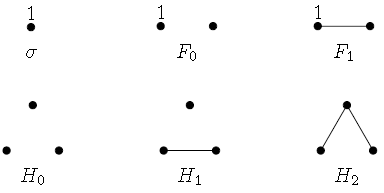
\includegraphics[width=7cm]{Figuras/fig2}\\
  \caption{$\sigma$-flags e grafos utilizados na prova do Teorema de Mantel.}\label{fig2}
\end{figure}

Nesta se\c{c}\~{a}o, um grafo admiss\'{\i}vel \'{e} um grafo que n\~{a}o cont\'{e}m $K_3$. Sobre os grafos admiss\'{\i}veis, considere $\sigma$, $\mathcal{F}^{\sigma}_{l} = \{ F_0,F_1 \}$, $\mathcal{H} = \{H_0,H_1,H_2\}$ como na figura \ref{fig2}. Considere tamb\'{e}m uma matriz sim\'{e}trica $2\times 2$ positiva semidefinida
\begin{equation*}
Q = \left[
  \begin{array}{cc}
    q_1 & q_2 \\
    q_2 & q_3 \\
  \end{array}
\right].
\end{equation*}

A fim de determinar os coeficientes $\alpha_{H}$ em \ref{aHQ} ser\'{a} necess\'{a}rio computarmos os valores de $\E{p(F_a,F_b;H[\bt])}$, para cada par $F_a,F_b \in \mathcal{F}_{l}^{\sigma}$. Tais valores est\~{a}o determinados na tabela \ref{tab2}.

\begin{table}
  \begin{tabular}{c|ccc}
                & $H_0$ & $H_1$ & $H_2$ \\ \hline
     $F_0,F_0$  & 1     & 0     & 0     \\
     $F_0,F_1$  & 1/3   & 1/3   & 0     \\
     $F_1,F_1$  & 0     & 1/3   & 1/3   \\
  \end{tabular}\caption{}\label{tab2}
\end{table}

Da\'{\i}, temos
\begin{equation}
   \begin{array}{rcccccc}
     \alpha_{H_0} & = & q_1 &+& \frac{2}{3}q_2 & & \\
     \alpha_{H_1} & = & & &\frac{2}{3}q_2 &+& \frac{1}{3}q_3 \\
     \alpha_{H_2} & = & & & & &\frac{1}{3}q_3\\
   \end{array}
\end{equation}

Temos tamb\'{e}m que $d(H_i) = i/3$, para $i = 0,1,2$. Portanto, o limitante superior em \ref{limitantes2} nos retorna
\begin{equation*}
\begin{array}{rcl}
     \pi(K_3) &\leq& \displaystyle{ \max \{d(H_0)  +  q_1 + \frac{2}{3}q_2, d(H_1) + \frac{2}{3}q_2 + \frac{1}{3}q_3, d(H_2) + \frac{1}{3}q_3 \}} \\
    &=& \displaystyle{ \max\{q_1 + \frac{2}{3}q_2, \frac{1}{3} + \frac{2}{3}q_2 + \frac{1}{3}q_3 ,\frac{2}{3} + \frac{1}{3}q_3 \} }.
\end{array}
\end{equation*}

Se tomarmos Q para ser
\begin{equation*}
Q = \left[
  \begin{array}{cc}
    1/2 & 0 \\
    0 & 1/2 \\
  \end{array}
\right],
\end{equation*}
obtemos
\begin{equation*}
     \pi(K_3) \leq \displaystyle{ \max\{\frac{1}{2}, \frac{1}{2} ,\frac{5}{6} \} }.
\end{equation*}

J\'{a} o problema \ref{SDPy} toma a seguinte forma:
\begin{equation}\label{SDPmantel}
\begin{aligned}
& \underset{y \in\mathbb{R}}{\text{minimize}} & & y \\
& \text{subject to} & & {\left\{\begin{array}{ccccccccc}
                           q_1  &+& \frac{2}{3}q_2  & &                 &-& y & \leq & 0 \\
                                & & \frac{2}{3}q_2  &+& \frac{1}{3}q_3  &-& y & \leq & -\frac{1}{3} \\
                                & &                 & & \frac{1}{3}q_3  &-& y & \leq & -\frac{2}{3} \\
                         \end{array}\right.
} \\
&&& \quad\quad Q \succeq 0,\;\;y \geq 0.
\end{aligned}
\end{equation}



\subsection{Resolvendo SDP}

%\section{Topologia das flag-\'{a}lgebras}

%--------------------------------------------------------------------------------------------------------------------------------------------------------
%   \'{I}NDICE REMISSIVO
%--------------------------------------------------------------------------------------------------------------------------------------------------------
%\printindex
%--------------------------------------------------------------------------------------------------------------------------------------------------------
%   BIBLIOGRAFIA
%--------------------------------------------------------------------------------------------------------------------------------------------------------
\bibliographystyle{plain}
\bibliography{Bibliografia}
%--------------------------------------------------------------------------------------------------------------------------------------------------------
%   FIM DO DOCUMENTO
%--------------------------------------------------------------------------------------------------------------------------------------------------------
\end{document} 